\end{multicols*}

\mysection{The Crux of Knowledge}{cruces-knowledge}

\flavor{Christ. Seven years of college down the drain. \\~ \Tilde "Bluto" Blutarsky, Animal House}


Order is the purpose of the Dream, and the ultimate servant of Order is science - humble, obedient, and aloof. Few have the patience and discipline to seduce it and bend it to their purpose. By mastering the Crux of Knowledge, you use learn the scientific art of \mybold{Leechcraft} to save lives and mend wounds using your \mybold{Ingenuity}.

    \begin{center}
    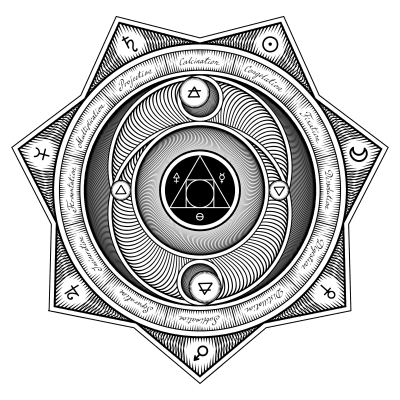
\includegraphics{cruces/CruxOfKnowledge}
    \end{center}

\mysubsection{Ingenuity}{cruces-knowledge-ingenuity}

    \begin{center}
        \myemph{Your Ingenuity starts at d4}
    \end{center}


Your \mybold{Ingenuity} is a Resource Die that represents your skill at using what's on hand to rehabilitate, revive, and restore through the practice of \mypg{Arcana:Leechcraft}{arcana-leechcraft}.  As your \UD moves \DCDOWN, you begin to run out of materials on hand - no more poultices, creams, salves, herbs, etc. You start with a \UDD{d4}, but can increase this die through \mypg{Advancement}{advancement}.


Your \MAX Ingenuity also affords you certain honorifics in "polite society", which may open doors among the wealthy and knowledgeable:


\myctrtable{Y Y}{
      \thead{Honorific} & \thead{Ingenuity} \\
    }{
      "Right Honorable" & d4  \\
      "Professor" & d6  \\
      "Doctor" & d8  \\
      "Maestro" & d10  \\
    }




\begin{multicols*}{2}
